%\documentclass[11pt, oneside]{book}
\documentclass[11pt, twoside, openright]{book}


%------------------------
%------- PAQUETES -------
%------------------------

% Establecemos el tamaño de página y márgenes
\usepackage[a4paper, total={6in, 8in}]{geometry}

% ----- Establecemos la distancia entre párrafos ------

% El paquete parskip no sólo añade espacio entre párrafos sino que elimina
% también la identación de la primera línea de % cada uno. Como no queremos
% esto último guardamos la conf. de la identación antes de cargar el paquete.
\edef\restoreparindent{\parindent=\the\parindent\relax}

% Cargamos el paquete
\usepackage{parskip}

% Restauramos la identación
\restoreparindent

%\setlength{\parskip}{1em} % Sustituido por las instrucciones anteriores
% -----------------------------------------------------

\usepackage[utf8]{inputenc}
\usepackage[british, spanish]{babel}
\usepackage[T1]{fontenc}

% Bibliografía
\usepackage[backend=bibtex,style=authoryear,citestyle=authoryear]{biblatex}
\usepackage{csquotes}

% Visualización de marcadores en el lector PDF
\usepackage{bookmark}

% \overset, numeración de teoremas y otras
\usepackage{amsmath}

% Para cambiar numeración de "enumerate"
\usepackage{enumitem}

% Para \mathbb etc.
\usepackage{amssymb}

% Para pseudocódigo
\usepackage{algpseudocode}
\usepackage{algorithm}

% Para código
\usepackage{listings}
\usepackage[table,xcdraw]{xcolor} % tambíen incluye colores para tablas.

% Para circuitos cuanticos. Requiere tener en el directorio el archivo qcircuit.sty
\usepackage{qcircuit}

\definecolor{codegreen}{rgb}{0,0.6,0}
\definecolor{codegray}{rgb}{0.5,0.5,0.5}
\definecolor{codepurple}{rgb}{0.58,0,0.82}
\definecolor{backcolour}{rgb}{0.95,0.95,0.92}

\lstdefinestyle{mystyle}{
    backgroundcolor=\color{backcolour},   
    commentstyle=\color{codegreen},
    keywordstyle=\color{magenta},
    numberstyle=\tiny\color{codegray},
    stringstyle=\color{codepurple},
    basicstyle=\ttfamily\footnotesize,
    breakatwhitespace=false,         
    breaklines=true,                 
    captionpos=b,                    
    keepspaces=true,                 
    numbers=left,                    
    numbersep=5pt,                  
    showspaces=false,                
    showstringspaces=false,
    showtabs=false,                  
    tabsize=2
}

\lstset{style=mystyle}

% Para inserción de imágenes
\usepackage{graphicx}

% Para definición de teoremas
\usepackage{amsthm}

% Para gráficos
\usepackage{tikz}
%\usetikzlibrary{arrows.meta} % Paquete para usar <-> como comandos para flechas en tikz, pero no me funciona :(

%------------------------
%------- TEOREMAS -------
%------------------------

\newtheorem{thm}{Teorema}[chapter] % Estilo de texto cursivo

\theoremstyle{definition} % Cambio del estilo de los teoremas a normal
\newtheorem{proposition}[thm]{Proposición}
\newtheorem{definition}[thm]{Definición}
\newtheorem{corolario}[thm]{Corolario}
\newtheorem{example}[thm]{Ejemplo}
\newtheorem{observation}[thm]{Observación}
\newtheorem*{lema}{Lema}
\newtheorem*{nota}{Nota}

%------------------------
%------- COMANDOS -------
%------------------------

% Conjuntos y constantes matemáticas
\newcommand{\R}{\mathbb{R}} % Reales
\newcommand{\C}{\mathbb{C}} % Complejos
\newcommand{\K}{\mathbb{K}} % Cuerpo K (reales o complejos)
\newcommand{\Sp}{\mathbb{S}} % Esfera
\newcommand{\e}{\mathrm{e}} % número e
\newcommand{\N}{\mathbb{N}} % Naturales
\newcommand{\Q}{\mathbb{Q}} % Racionales
\newcommand{\B}{\mathcal{B}} % Base

\newcommand{\qsh}{\textsf{Q}\texttt{\#}} % Q#
\newcommand{\csh}{\textsf{C}\texttt{\#}} % C#

\newcommand{\orden}[1]{\mathcal{O}\left(#1\right)}

\newcommand{\oversim}[1]{\overset{_\sim}{#1}} % Para poner ~ sobre algo

% Para poner datos encima y/o debajo de implica
\newcommand{\ximplies}[2]{\underset{#2}{\overset{#1}\implies}}
\newcommand{\xiff}[2]{\underset{#2}{\overset{#1}\iff}}
\newcommand{\ximpliedby}[2]{\underset{#2}{\overset{#1}\impliedby}}

% Producto escalar y norma
\newcommand{\dotproduct}[2]{\langle#1,#2\rangle}
\newcommand{\norm}[1]{\left|\left|#1\right|\right|}

% Notación de Dirac -- SUSTITUIR POR PAQUETE DE LUIS
\newcommand{\ket}[1]{\left|#1\right\rangle}
\newcommand{\bra}[1]{\left\langle#1\right|}
\newcommand{\braket}[2]{\left\langle#1|#2\right\rangle}

% Vectores
\newcommand{\twovector}[2]{\begin{pmatrix} #1 \\ #2 \end{pmatrix}} % Vector de dim 2

% Funciones e info debajo de funciones
\newcommand{\function}[3]{#1\colon #2\longrightarrow #3}
\newcommand{\xfunction}[4]{\underset{#4}{{#1\colon #2\longrightarrow #3}}}

% Funcion que transforma estados |0> y |1>
\newcommand{\gatetwo}[3]{#1\colon \begin{matrix}\ket0&\longrightarrow& #2\\ \ket1&\longrightarrow& #3\end{matrix}}

% Funcion que transforma estados |00>, |01>, |10> y |11>
\newcommand{\gatefour}[5]{#1\colon \begin{matrix} \ket{00}&\longrightarrow& #2\\ \ket{01}&\longrightarrow& #3\\ \ket{10}&\longrightarrow& #4\\ \ket{11}&\longrightarrow& #5 \end{matrix}}

% Introducir información debajo de igualdad
\newcommand{\equals}[2]{\underset{#2}{\underset{\shortparallel}{#1}}}

% Comandos para palabras dentro de ecuaciones $ $ o \[ \]
\newcommand{\y}{\mathrm{\ y\ }}
\newcommand{\cte}{\mathrm{cte}}
\newcommand{\rg}{\mathrm{rg}}
\newcommand{\id}{\mathrm{id}}

%Página en blanco NO numerada
\newcommand\blankpage{%
    \null
    \thispagestyle{empty}%
    \addtocounter{page}{-1}%
    \newpage}


\renewcommand{\baselinestretch}{1.1}

\title{Computación cuántica: Pruebas de mutación}
\author{Luis Aguirre \& Javier Pellejero}

\bibliography{bibliography/bibliography}


\newcommand{\jicomment}[1]{\textcolor{red}{#1}}

\tracingpages1
\tracingoutput1

\makeatletter
\def\cleardoublepage{\clearpage\if@twoside \ifodd\c@page\else
    \hbox{}
    \thispagestyle{plain}
    \newpage
    \if@twocolumn\hbox{}\newpage\fi\fi\fi}
\makeatother \clearpage{\pagestyle{plain}\cleardoublepage}

\begin{document}

% Portada, página en blanco\emph{•}, cita e índice
%----------------------------------
%Inicio portada
	\begin{titlepage}
\begin{center}
\vspace*{+0.15in}
%Título español
\textbf{\textsc{\begin{LARGE}Inferencia y verificación de propiedades en sistemas ciber-físicos estocásticos\end{LARGE}}}


%Título inglés
\textbf{\textsc{\begin{LARGE}Título en inglés: Inference and verification of properties in stochastic cyber-physical systems\end{LARGE}}}

\vspace*{+0.15in}

\textsc{\textbf{\begin{large} Director: José Ignacio Requeno\end{large}}\\}
\vspace*{0.1in}

\textsc{\textbf{\begin{normalsize}Autores: Javier Romero Flores (GIC) \&  Dmytro Vernyuk (GII)\end{normalsize}}\\}

\begin{figure}[htb]
\begin{center}

\includegraphics[width=7.8cm]{chapters/complu}\\\ \\\ \\

\textsc{\begin{large}Trabajo de fin de grado del Grado en Ingeniería de Computadores e Ingeniería Informática\end{large}}\\\ \\

\textsc{\begin{Large}Facultad de Informática\end{Large}}\\\ \\

\textsc{\textbf{\begin{LARGE}Universidad Complutense de Madrid\end{LARGE}}}\\
\end{center}
\end{figure}

Curso 2021-2022
\end{center}
\end{titlepage}
% Fin portada
%-------------------------------------------------------

\blankpage

\pagenumbering{Roman} % para comenzar la numeracion de paginas en numeros romanos
	\chapter*{}
\begin{flushright}
\textit{I ain’t no physicist but I know what matters.}\\\ \\ – Popeye el Marino
\end{flushright}

% Resumen, abstract...
\chapter*{}

\section*{Resumen (español)}
Este Trabajo de Fin de Grado tiene principalmente como objetivo la ampliación de las capacidades de análisis de las herramientas para la verificación de los sistemas ciberfísicos en tiempo de ejecución. Los requisitos de la verificación están expresados en  Signal Temporal Logic (STL), un tipo de lógica temporal enfocada al análisis de señales analógicas o reales. La lógica temporal es su vez un tipo de lógica modal que nos permite expresar propiedades sobre un estado o una secuencia de estados del sistema. La ampliación consiste en añadir dos nuevos operadores lógicos, la derivada (tendencias) y la integral (acumulaciones).

La segunda parte del proyecto consiste en probar el buen funcionamiento de una biblioteca de minería de datos ya existente para casos paramétricos con los nuevos operadores y ofrecer una nueva interfaz gráfica para una interacción mas fácil tanto con STL como con la biblioteca de minería.

\textbf{Palabras Clave}:
\begin{itemize}
\item STL
\item Lógica Temporal
\item C++
\item Python
\item Interfaz Gráfica
\item PyQt
\item Minería de Datos 
\end{itemize}
\newpage

\section*{Abstract (English)}
\begin{otherlanguage}{british}
The purpose of this Final Degree Project is mainly to expand the analysis capabilities of the tools for the verification of cyber-physical systems at runtime. The verification requirements are expressed in Signal Temporal Logic (STL), a type of temporal logic focused on the analysis of analog or real signals. Temporal logic is in turn a type of modal logic that allows us to express properties about a state or a sequence of states of the system. The extension consists of adding two new logical operators, the derivative (trends) and the integral (accumulation).

The second part of the project consists of testing the functionality of an existing data mining library for parametric cases with the new operators and offering a new graphical interface for easier interaction with both STL and the mining library.
\end{otherlanguage}

\textbf{Keywords}:
\begin{itemize}
\item STL
\item Temporal Logic
\item C++
\item Python
\item GUI
\item PyQt
\item Data Mining
\end{itemize}


\chapter*{Prefacio}

Prefacio.

\tableofcontents % Índice

\mainmatter % Empieza a numerar en números arábigos 

%TODO Glosario con acrónimos y definiciones?
% Introducción
%\chapter{Introducción histórica}
%
%\section{Antecedentes históricos y actualidad (español)}
%Primera sección.
%
%\section{Historical and current background (English)}
%
%\begin{otherlanguage}{british}
%En inglés
%\end{otherlanguage}

\chapter{Introducción}

\section{Sistemas ciberfísicos}
Los sistemas ciberfísicos son un tipo especial de sistemas en tiempo real que combinan un micro controlador o programa software, representado mediante una máquina de estados discretos, con uno o varios sensores que interactúan sobre una variable física. Ejemplos de este tipo de entornos son los ordenadores de a bordo que regulan la velocidad de crucero de un vehículo, o el piloto automático que controla la altitud y trayectoria de un avión.

Garantizar el correcto funcionamiento de estas plataformas es crucial, ya que un mal funcionamiento conlleva una reducción del comfort por parte de los usuario o, incluso, la pérdida de vidas humanas. Una manera de asegurarlo es mediante el uso de técnicas de verificación formal. Las técnicas de verificación en tiempo de ejecución \cite{STTT_RV_21} (\emph{runtime verification} en inglés) implementan un monitor que supervisa que la ejecución actual cumple con los requisitos especificados. Los monitores actúan como guardianes, alertando al usuario cuando la ejecución se desvía del comportamiento deseado e, incluso, implementando contramedidas para revertir ese hecho y redirigir el sistema hacia un estado saludable. 

Existen diversos formalismos para definir los comportamientos deseados y no deseados. Los requisitos se pueden expresar operacionalmente, mediante algún tipo de autómata de estados finito, o declarativamente, mediante una descripción lógico-matemática. Dentro de esta segunda categoría, la lógica temporal es un tipo de lógica modal que expresa propiedades sobre un \emph{estado} en particular del sistema, o sobre los \emph{caminos} (es decir, secuencia de estados) que atraviesa. En este trabajo utilizaremos Signal Temporal Logic \cite{STL}, un tipo de lógica temporal enfocada al análisis de señales analógicas o reales.

\section{Lógica Temporal}

Si navegamos por internet o buscamos en los libros acerca de qué es la lógica temporal tarde o temprano daremos con una cita del filósofo alemán Kant que cita: 

\begin{center}
\textit{"la posibilidad de principios apodícticos de las relaciones del tiempo, o axiomas del tiempo en general. Tiene una sola dimensión: los distintos tiempos no son simultáneos, sino sucesivos"}
\end{center}

Y, aunque quizás sacado de todo contexto, es un buen primer comienzo para explicar acerca de qué es el tiempo y por consiguiente qué tiene que ver la lógica con éste. Y es que Kant quería expresar que el tiempo es algo que va ocurriendo constantemente, es un conjunto de hechos que juntos transcurren en una dirección y conforman el tiempo, pues bien, teniendo en cuenta esta idea podemos llegar a comprender y diferenciar la lógica temporal. 

La lógica proposicional no tiene la persepción de tiempo, en este tipo de lógica tenemos hechos que son verdaderos o falsos, que unidos pueden transformarse en verdad o no, pero nunca individualmente cambian su valor, por ejemplo si decimos que:

\begin{center}
s = ``El día está soleado''
\end{center}

Este argumento será eterno individualmente, aún asi realicemos operaciones con él como negarlo $\neg{s}$, todo el argumento se verá afectado en todo momento:

\begin{center}
$\neg{s}$ = ``El día no está soleado''
\end{center}

Pero como todos podemos percibir, en la realidad esto no sucede, en otras palabras, puede que "no todo el día esté soleado", quizás si por la mañana y no por la tarde o visceversa, esto es lo que trata de expresar la lógica temporal. En un momento determinado una expresión puede ser verdad mientras que en otra hora, minuto, segundo, o cuálquier otra unidad que utilicemos para medir el tiempo , puede cambiar y tener un valor diferente. 

\section{Objetivos}

Los objetivos de este proyecto son:

\begin{itemize}
\item extender las capacidades de la lógica temporal STL para expresar propiedades que involucren \textit{tendencias} (derivadas), o \textit{acumulaciones} (integrales),    
\item implementar esos nuevos operadores lógicos en las herramientas software actuales; y, por último,
\item proporcionar una interfaz de usuario amigable que facilite la interacción con dichas herramientas.  
\end{itemize}

En particular, los objetivos de proyecto se han plasmado en contribuciones concretas sobre las siguientes herramientas software preexistentes:

\begin{itemize}
\item \textbf{STLEval} \cite{StlEval}: Es una herramienta capaz de procesar especificaciones en STL y evaluarlas sobre una señal real. Ha recibido la implementación de los nuevos operadores lógico temporales que calculan derivadas e integrales sobre una señal.
\item \textbf{ParetoLib} \cite{ParetoLib}: Es una biblioteca de de minería que aprende las configuraciones (in)válidas del sistema monitorizado, expresadas como plantillas o especificaciones paramétricas en STL. ParetoLib internamente se conecta con STLEval para la ejecución de los cálculos. Ha recibido una actualización de los binarios y bibliotecas DLL de STLEval que empaqueta de forma conjunta con el resto de la biblioteca, así como la interfaz gráfica de usuario. La nueva interfaz gráfica de usuario permite interaccionar tanto con la biblioteca de aprendizaje como indirectamente con la herramienta STLEval.
\end{itemize}

\section{Organización del documento}

El documento está dividido en 4 capítulos. En el capítulo \ref{cha:stl} detallaremos la semántica e implementación de los nuevos operadores lógicos. El capítulo \ref{cha:gui} está dedicado a la nueva interfaz gráfica de usuario. Finalmente, continuamos con las conclusiones más relevantes del proyecto en el capítulo \ref{cha:concl}, donde se incluye también ideas para el trabajo futuro. %Los anexos X recogen imágenes, código adicional, $\ldots$.

\section{Planificación temporal y esfuerzo}

Este proyecto tuvo una duración de 8 meses y ha sido realizado por dos estudiantes a tiempo parcial, Dmytro Vernyuk (GII) y Javier Romero Flores (GIC), con una dedicación media de 3 horas al día. Los alumnos han estado tutorados por José Ignacio Requeno mediante reuniones semanales. Se han modificado o creado aproximadamente 1300 líneas de código, que están repartidas entre las dos herramientas software actualizadas y la nueva interfaz gráfica de usuario. El código desarrollado en este proyecto puede consultarse en ramas dedicadas a las nuevas funcionalidades de los correspondientes repositorios web (rama \textit{derivative} de STLEval y rama \textit{GUI} de ParetoLib). El proyecto arrancó el 13 de septiembre del 2021, ha durado 8 meses y ha constado de 4 fases.

\subsection{Primera - Investigación}
El proyecto se inició con una primera fase de investigación, donde nos dedicamos a adquirir los conocimientos teóricos necesarios para el trabajo: leer información sobre qué es la lógica temporal y la principal diferencia con otras lógicas modales. Recurrimos tanto al material proporcionado por el instructor como al material externo disponible para aprender las principales definiciones y sintaxis básicas. 

Ésta fue la parte más complicada de todo el trabajo no sólo por la dificultad teórica de la información especializada en el ámbito de la verificación, sino también por el cambio de paradigma que supone comprender el concepto principal de ésta lógica: que una afirmación se puede convertir en negación dependiendo del instante en el que se evalúa la expresión.
	
\subsection{Segunda - Documentación}

	Después de adquirir los conocimientos teóricos previos necesarios para la comprensión de las funcionalidades a implementar, continuamos con la lectura de la documentación de las bibliotecas y herramientas software que debíamos extender: su arquitectura software y jerarquía de clases. Dedicamos gran parte del esfuerzo a estudiar la definición de los operadores de derivación e integración propuestos en la literatura científica, y su posterior codificación e incorporación a la herramienta software STLEval.
	
	En esta fase, nuestra mayor dificultad fue 1) la labor de aprendizaje de la estructura interna del código de STLEval, y 2) la adquisición y aplicación de las nociones de derivación e integración sobre señales temporales.

\subsection{Tercera - Implementación}

	Implementamos las operaciones de derivación e integración de señales temporales en la herramienta software STLEval. Completamos esta tarea con un conjunto de pruebas sobre señales temporales con características \textit{benignas} que nos facilitaron ejecutar tests de validación: por ejemplo, la integral de una señal periódica (sinusoidal o triangular) simétrica sobre el eje horizontal debe ser cero en determinados intervalos.

\subsection{Cuarta - Diseño y Finalización}

	Como última tarea implementamos la interfaz gráfica de la aplicación, partiendo de un primer boceto que estabilizamos al cabo de dos reuniones. La tarea más complicada de este proceso fue la conexión entre los diferentes componentes de la interfaz con los métodos propios de las herramientas STLEval y ParetoLib, que ejecutan toda la lógica del programa.
	
	La conexión con STLEval se realizó mediante una API preexistente en C++ que ya estaba integrada en Python a través de la biblioteca ParetoLib. Este hecho, la posibilidad de acceder tanto a la biblioteca de minería ParetoLib como indirectamente a la herramienta STLEval, motivó la elección de Python como lenguaje de programación para el diseño de las ventanas de usuario. La facilidad de uso del lenguaje así como la cantidad de bibliotecas auxiliares para el tratamiento de datos con las que extender las funcionalidades de la interfaz en el futuro contribuyeron también a esta decisión.
	


\section{Organización de Equipo}

Debido a la dificultad teórica de este proyecto, decidimos realizar las tareas de manera conjunta: todos los apartados de este proyecto a excepción de la labor de documentación se realizaron a la par por ambos integrantes del equipo. 

La planificación coincide con las fases del proyecto, indicamos las fechas exactas en el siguiente gráfico.

\begin{figure}
\centering
  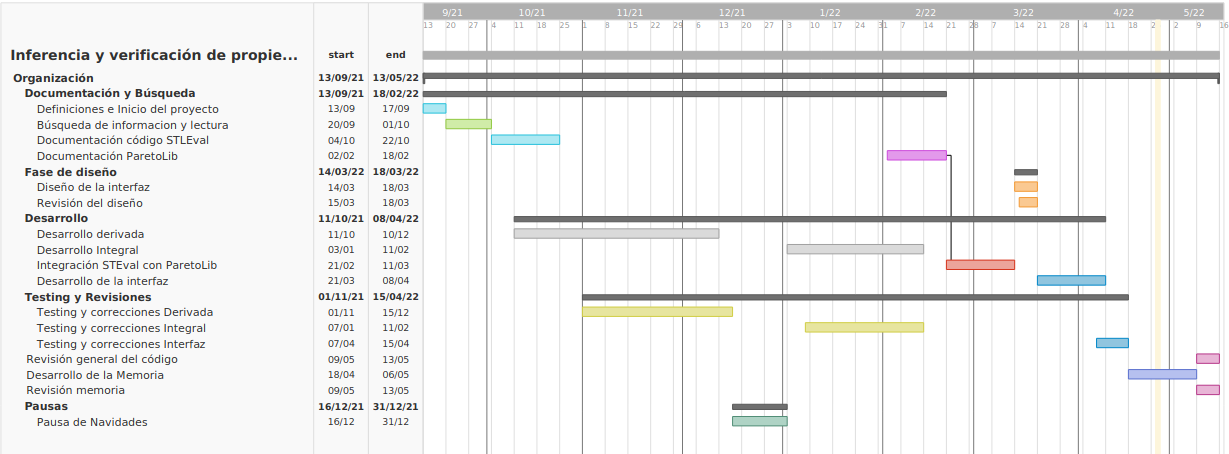
\includegraphics[width=.9\linewidth ,angle = 90,scale = 1.2]{images/gant}
\caption{Diagrama de Gantt.}
\label{fig:gant}
\end{figure}

\chapter{Introduction}

\section{Cyber-physical system}
Cyber-physical systems are a special type of real-time systems that combine a microcontroller or software program, represented by a discrete state machine, with one or more sensors that interact with a physical variable. Examples of this type of environment are the on-board computers that regulate the speed of a vehicle, or the autopilot that controls the altitude and trajectory of an aircraft.

Ensuring the proper functioning of these platforms is crucial, since a malfunction leads to a reduction in user comfort or even the loss of human lives. One way to ensure this is through the use of formal verification techniques. Runtime verification techniques \cite{STTT_RV_21} implement a monitor that monitors that the current execution meets specified requirements. Monitors act as keepers, alerting the user when execution deviates from desired behavior and even implementing countermeasures to reverse that fact and redirect the system back to a healthy state.

There are various formalisms to define desired and undesired behaviors. Functional requirements can be expressed operationally, through some kind of finite state automaton, or declaratively, through a logical-mathematical description. Within this second category, temporal logic is a type of modal logic that expresses properties about a particular \emph{state} of the system, or about the \emph{paths} (ie, sequence of states) that it traverses. In this work we will use Signal Temporal Logic \cite{STL}, a type of temporal logic focused on the analysis of analog signals.

\section{Objectives}

The objectives of this project are:

\begin{itemize}
\item Extend the capabilities of temporal logic to express properties involving \textit{trends} (derivatives), or \textit{accumulations} (integrals), 
\item Implement these new logical operators in current software tools, and
\item Provide a friendly user interface that facilitates interaction with said tools.
\end{itemize}


In particular, the project objectives have been translated into concrete contributions to the following pre-existing software tools:

\begin{itemize}
\item \textbf{STLEval} \cite{StlEval}: It is a tool capable of processing STL specifications and evaluating them on a real signal. It has received the implementation of the new temporal logic operators that calculate derivatives and integrals on a signal.
\item \textbf{STLEval} \cite{StlEval}: It is a mining library that learns the (in)valid configurations of the monitored system expressed as templates or parametric specifications in STL.
ParetoLib internally interfaces with STLEval for the execution of the calculations. It has received an update of the STLEval binaries and DLL libraries which package together with the rest of the library, as well as the graphical user interface. The new GUI allows to interact both with the learning library and indirectly with the STLEval tool.
\end{itemize}

\section{Document Organization}

The document is divided into 4 chapters. In the chapter \ref{cha:stl} we will detail the semantics and implementation of the new logical operators. The \ref{cha:gui} chapter is dedicated to the new graphical user interface. Finally, we continue with the most relevant conclusions of the project in the chapter \ref{cha:concl}, and sketch some ideas for the future work. %Finally $\ldots$.

\section{Time schedule and effort}
This project lasted 8 months and was carried out by two part-time students, Dmytro Vernyuk (GII) and Javier Romero Flores (GIC), with an average dedication of 3 hours per day. The students have been tutored by José Ignacio Requeno through weekly meetings. Approximately 1300 lines of code have been modified or created, which are distributed between the two updated software tools and the new graphical user interface.
graphical user interface. The code developed in this project can be consulted in the new functionalities of the corresponding web repositories (\textit{derivative} branch of STLEval and \textit{GUI} branch of ParetoLib). The project started on September 13, 2021, and has consisted of 4 phases.


\subsection{First - Research}
The project started with a first phase of research, where we dedicated ourselves to theoretical knowledge necessary for the work: reading information about what is temporal logic and the main difference with other modal logics.
We resorted both to the material provided by the instructor and to the external material available to learn the main definitions and basic syntax.
This was the most complicated part of the whole work not only because of the theoretical difficulty of the specialized information in the field of 
but also because of the paradigm shift involved in understanding the main concept of this logic: that an assertion can become a negation depending on the instant at which the expression is evaluated.


\subsection{Second - Documentation}
After acquiring the previous theoretical knowledge necessary for the understanding of the functionalities to be implemented, we continued with the reading of the documentation of the libraries and software tools to be extended: their software architecture and class hierarchy. We devoted a great deal of effort to study the definition of the derivation and integration operators proposed in the scientific literature, and their subsequent coding and incorporation into the STLEval software tool.

\subsection{Third - Implementation}
We implemented the operations of derivation and integration of time signals in the STLEval software tool. We completed this task with a set of tests on time signals with \textit{benign} characteristics that facilitated us to run validation tests: for example, the integral of a periodic signal (sinusoidal or triangular) symmetric about the horizontal axis should be zero in  certain intervals.

\subsection{Fourth - Design and Completion}
As a last task we implemented the graphical interface of the application, starting from a first sketch that we stabilized after two meetings. The most complicated task of this process was the connection between the different components of the interface with the methods of the STLEval and ParetoLib tools, which execute all the program logic.

The connection with STLEval was made through a pre-existing API in C++ that was already integrated in Python through the ParetoLib library. This fact, the possibility of accessing both the ParetoLib mining library and the STLEval tool indirectly, motivated the choice of Python as the programming language for the design of the user windows. The ease of use of the language as well as the number of auxiliary libraries for data processing with which to extend the functionalities of the interface in the future also contributed to this decision.

\section{Team Organization}
Due to the theoretical difficulty of this project, we decided to carry out the tasks jointly: all the sections of this project, except for the documentation work, were carried out at the same time by both members of the team.
The planning coincides with the phases of the project, the exact dates are shown in the following chart.

\begin{figure}
\centering
  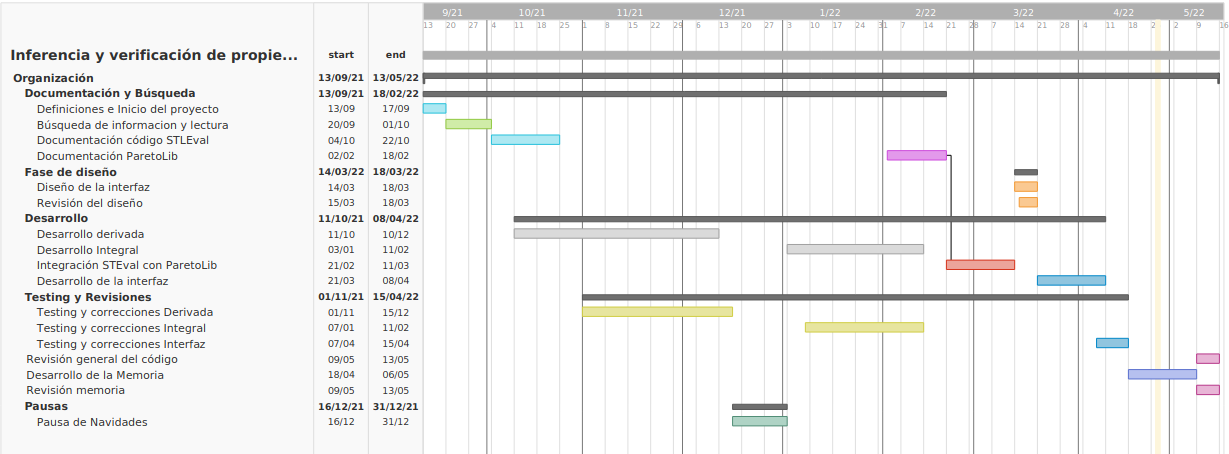
\includegraphics[width=.8\linewidth ,angle = 90,scale = 1]{images/gant}
\caption{Diagrama de Gantt.}
\label{fig:gant2}
\end{figure}

% Varios capitulos
% Nuevos operadores para STL
\chapter{Nuevos operadores para STL}
\label{cha:stl}

\section{Signal Temporal Logic}
% Definición, sintaxis y semántica de los operadores.
\textit{Signal Temporal Logic} (STL) \cite{STL} es un tipo de lógica temporal especializada en el análisis de señales reales analógicas. STL permite expresar características sobre la evolución de algún atributo físico, como la velocidad o temperatura. Por tanto, como punto de partida, STL requiere una muestra o traza de ejecución sobre la que comprobar las hipótesis.

La lógica distingue dos tipos de situaciones: propiedades que se satisfacen en un \textit{estado} o momento puntual de la traza de ejecución, o propiedades de \textit{camino} que se evalúan a lo largo de una secuencia de eventos. STL proporciona operadores para recorrer los diferentes estados del sistema y comprobar en qué momentos se cumplen las propiedades.

Por ejemplo, la proposición atómica $v > 120$ mostraría los instantes en los que la velocidad supera los $120$. Los operadores de camino enriquecerían esa expresión para analizar si la velocidad se sobrepasa puntualmente en algún momento (\textbf{F})uturo del viaje, (\textbf{G})eneralmente a lo largo de todo el recorrido, o permanece constante hasta (\textbf{U}ntil) que se incrementa a un nuevo valor. 

Formalmente, la gramática básica de STL comprende los siguientes operadores:

$$ \varphi \ := \ \mu \ |\ \neg \varphi \ |\ \varphi_{1} \lor \varphi_{2} \ |\ \varphi_{1} U_{[t_1, t_2]} \varphi_{2}$$

Donde $\mu$ representa las proposiciones atómicas, en forma de desigualdades sobre la señal muestreada (p.ej., $\mu := v > 120$); y $\varphi$ las especificaciones sobre los caminos. El resto de los operadores se componen a partir de los operadores precedentes, donde $t_1, t_2 \in \mathbb{R}_{\geq 0}$ son marcas temporales que definen el intervalo de monitorización respecto al instante inicial, siendo $t_1 \geq t_2$. 

% Operador futuro y general

% $$ F_{[a,b]} \varphi \equiv \top U_{[a,b]} \varphi $$
% $$ G_{[a,b]} \varphi \equiv \neg F_{[a,b]} \neg \varphi $$

\begin{align*}
F_{[a,b]} \varphi \equiv \top U_{[a,b]} \varphi & &
G_{[a,b]} \varphi \equiv \neg F_{[a,b]} \neg \varphi
\end{align*}

Existen versiones extendidas que permiten analizar aspectos cuantitativas con STL, por ejemplo, los valores máximos/mínimos \cite{TACAS_19} o integrales en un intervalo, o calcular la derivada en un punto \cite{Stl_Der_Int}.


Las especificaciones en STL se \textit{compilan} en un monitor que supervisa la ejecución del sistema (p. ej., el sensor de velocidad de un vehículo). Algunos intérpretes de STL son AMT \cite{AMT2} (sintaxis básica) y STLEval \cite{StlEval} (sintáxis básica y operadores de min/max). En este proyecto, implementaremos en STLEval los operadores cuantitativos de STL que permiten calcular integrales y derivadas sobre una señal, según la definición propuesta en \cite{Stl_Der_Int}.

\section{STLEval}
%Lenguaje utilizado en STLEval (C++), etc.
STLEval es una herramienta capaz de manejar tanto expresiones STL básicas, que devuelven señales Booleanas, como ciertas extensiones cuantitativas, que transforman la señal de entrada en una nueva señal continua (operadores de min/max). Por estos motivos, así como su eficiencia (está escrita en en C++) STLEval se ha tomado como punto de partida para implementar los operadores cuantitativos de STL que permiten calcular integrales y derivadas sobre una señal, según la definición propuesta en \cite{Stl_Der_Int}.

% Muestreo de la señal. Representación interna en STLEval.
Internamente, STLEval representa una señal como una serie temporal, es decir, una sucesión de pares \textit{(clave, valor)} donde la \textit{clave} es una marca temporal y el \textit{valor} representa la magnitud física en ese momento. La imagen \ref{fig:senal} ilustra la señal original y su representación interna en STLEval. 

\begin{figure}
\centering
  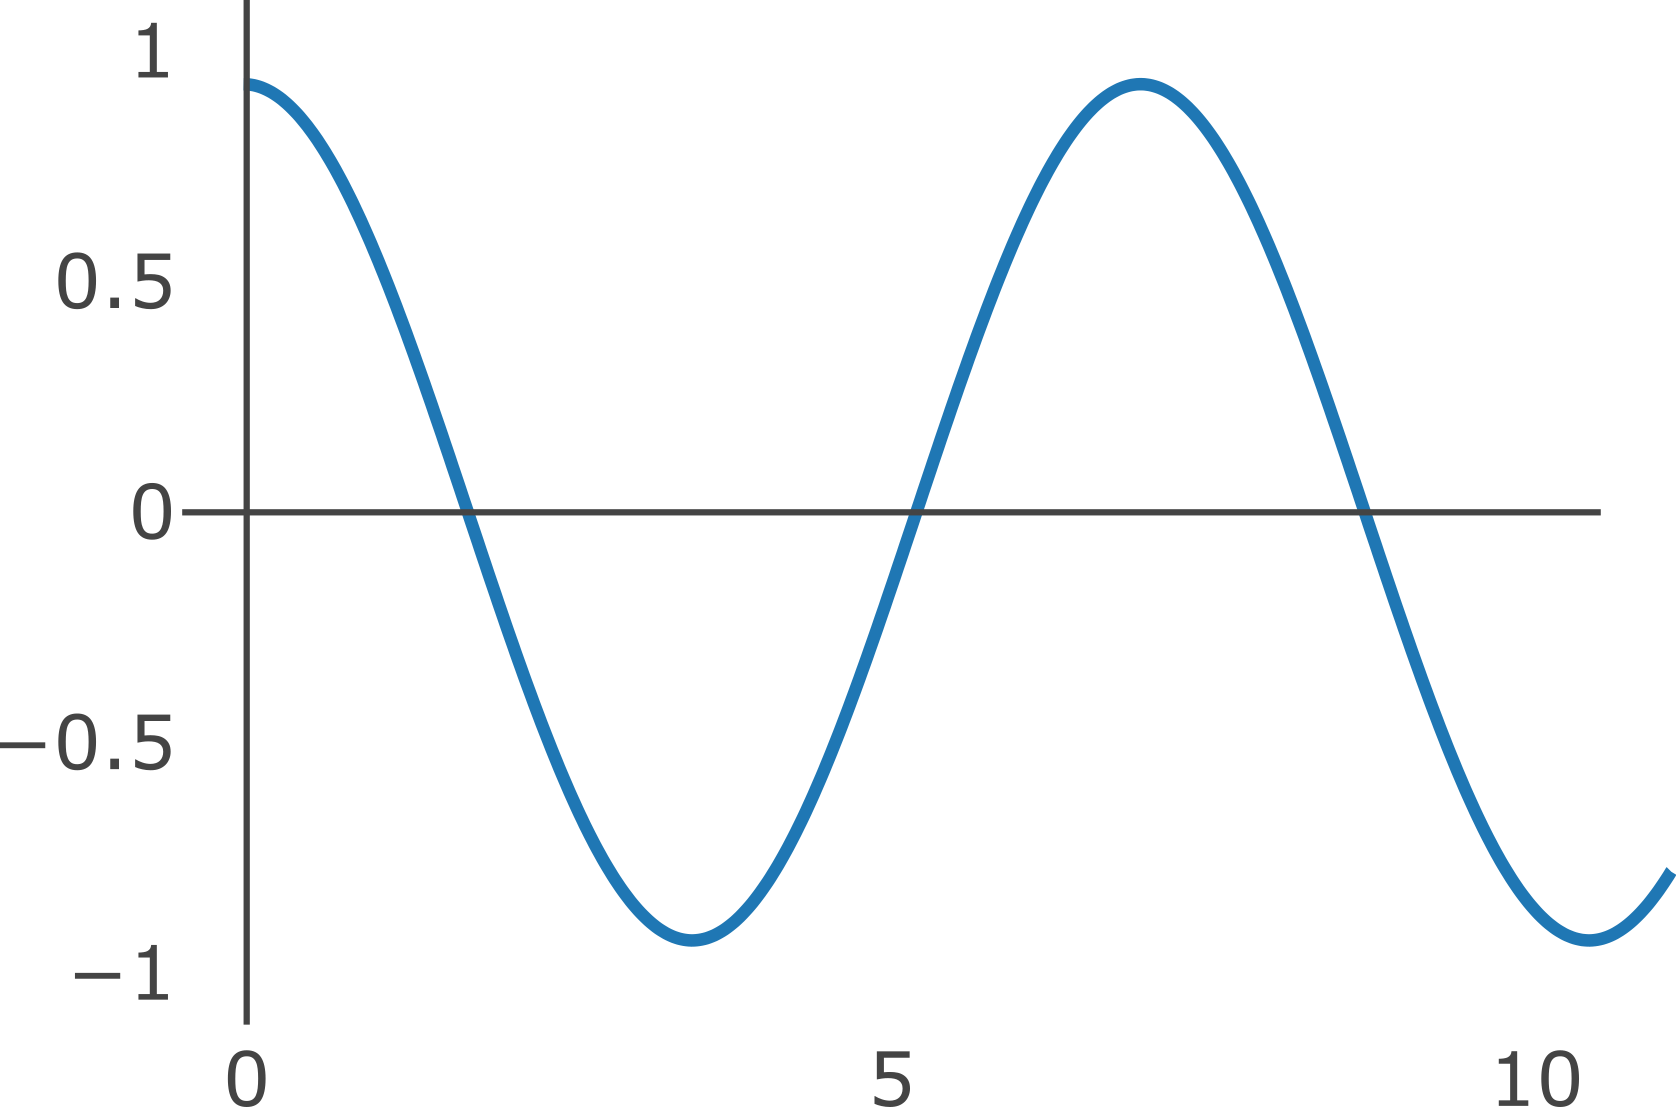
\includegraphics[width=.4\linewidth]{images/senal_original} \hfill
  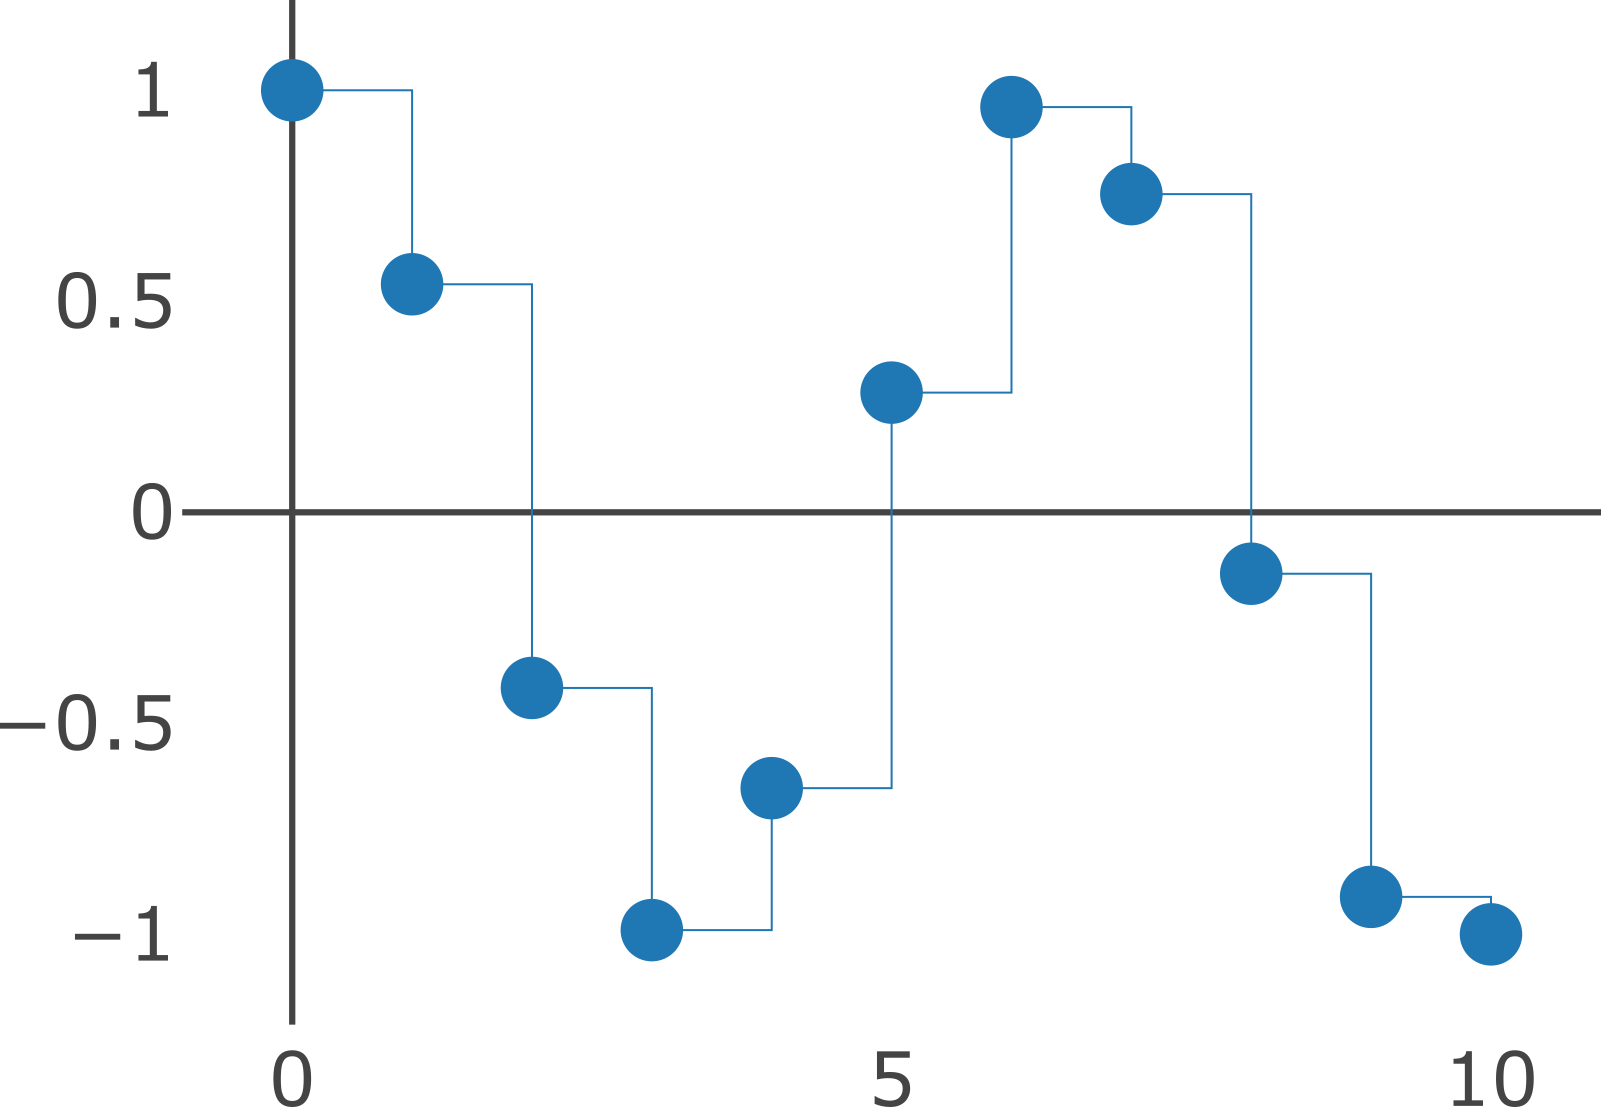
\includegraphics[width=.4\linewidth]{images/senal_muestreada}
\caption{Señal original y su reconstrucción.}
\label{fig:senal}
\end{figure}

\section{Definición de los nuevos operadores}

El cálculo de la derivada e integral se aproximan mediante las siguientes expresiones matemáticas, donde $\mathbf{x}$ representa la señal completa, $\mathbf{x}_{\tau}$ es el valor de la señal en el instante $\tau$, y $\mu^d_{+}$ ($\mu^d_{-}$) representan la aproximación de la derivada por la derecha (izquierda) del instante temporal en cuestión:

\begin{align*}
\mu^d_{+} &= \frac{dg(\mathbf{x})}{dt^+} \geq c & & \mu^i_{[a,b]} = \int^{b}_{a} g(\mathbf{x}_{\tau}) \delta \tau \geq c \\
\mu^d_{-} &= \frac{dg(\mathbf{x})}{dt^-} \geq c &
\end{align*}

Dado que internamente STLEval representa las señales reales como una serie numérica de tiempo discreto, aproximamos como:

\begin{align*}
\mu^d_{+} &= g(\mathbf{x}_{(k + 1) \delta t}) - g(\mathbf{x}_{k \delta t}) \geq c \delta t & & \mu^i_{[a,b]} = \sum^{k + b / \delta t - 1}_{k' = k + a / \delta t} g(\mathbf{x}_{k' \delta t}) \delta t \geq c \\
\mu^d_{-} &= g(\mathbf{x}_{k \delta t}) - g(\mathbf{x}_{(k - 1) \delta t}) \geq c \delta t & 
\end{align*}

Gráficamente, la derivada se interpreta como la pendiente entre dos puntos consecutivos de la señal; y la integral como el sumatorio del área de los rectángulos con base  $\delta t$ contenidos en el intervalo (Figura \ref{fig:der_int}). 

\begin{figure}
\centering
  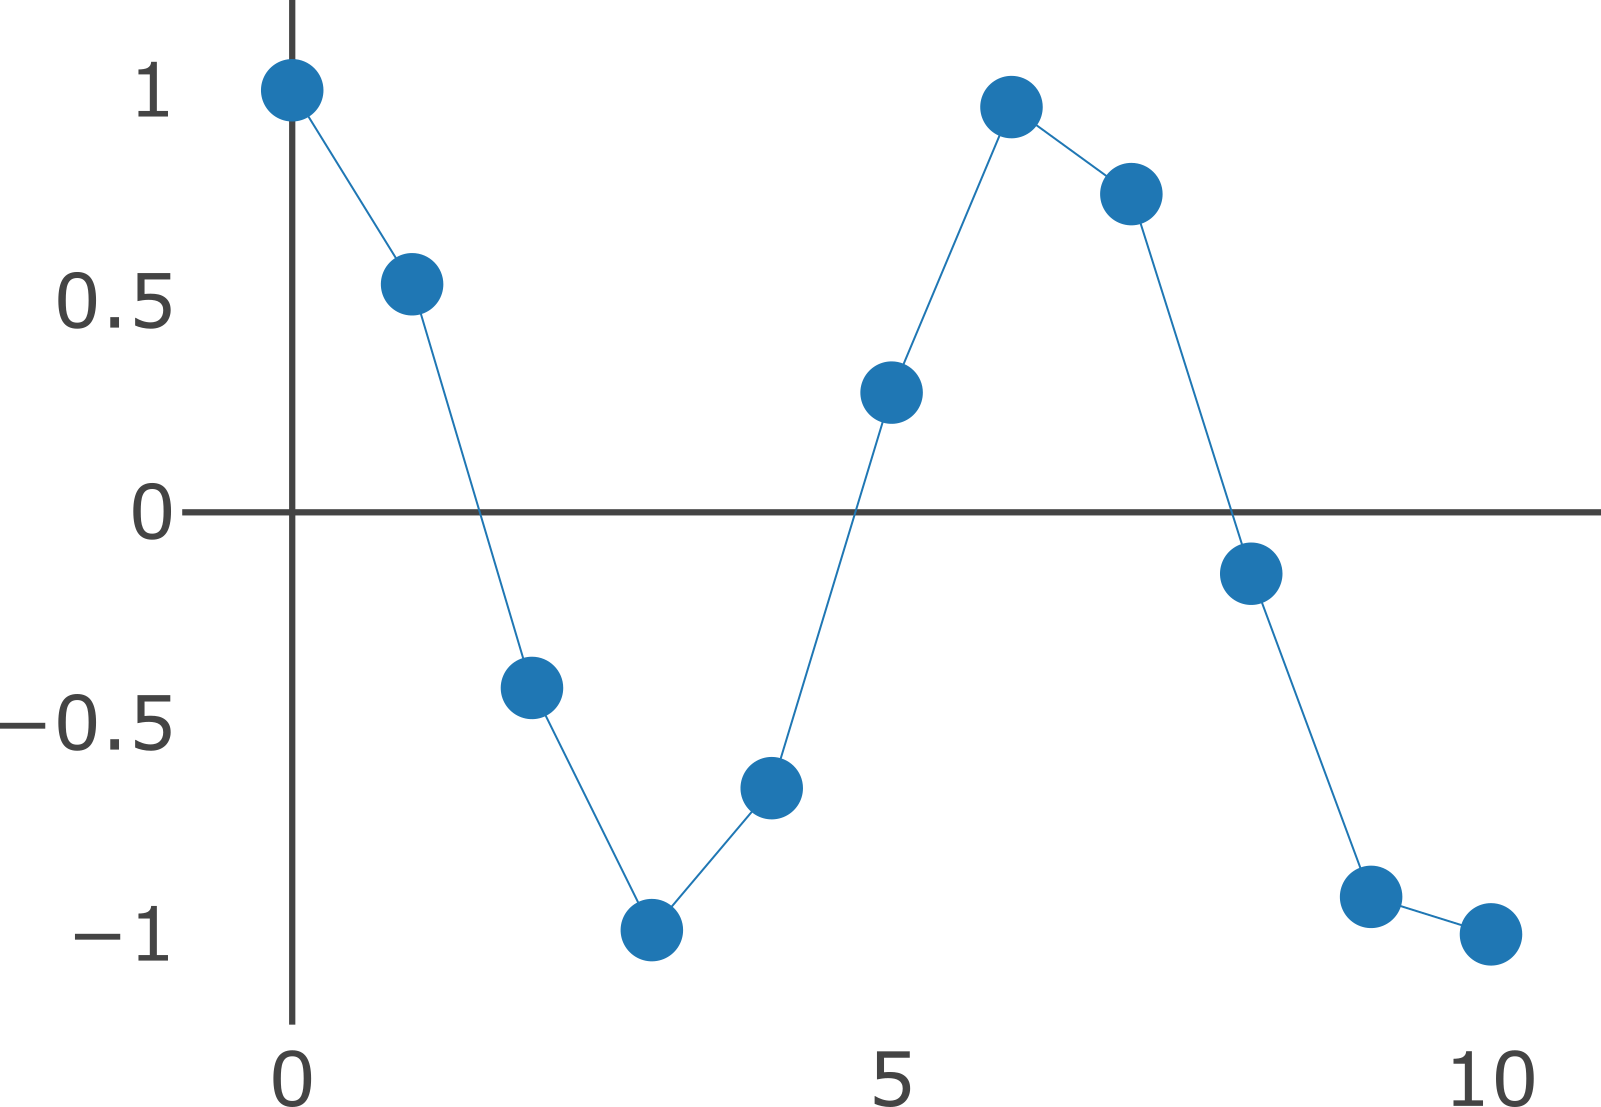
\includegraphics[width=.4\linewidth]{images/derivada} \hfill
  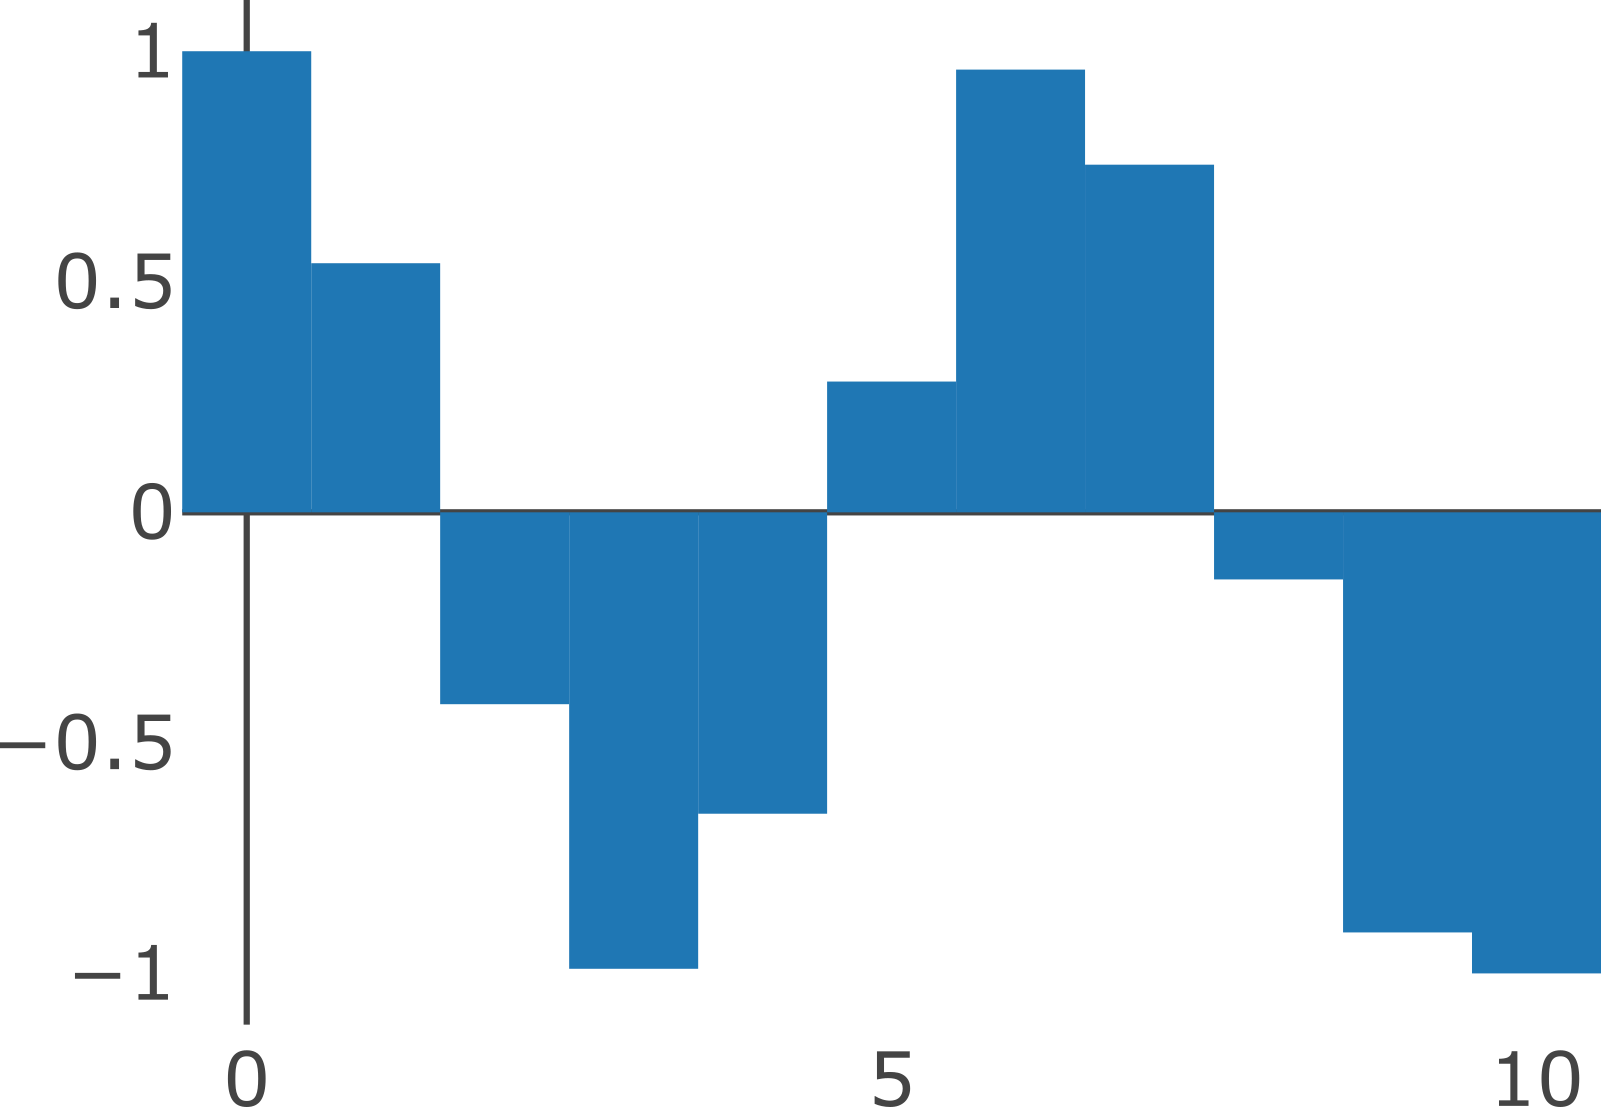
\includegraphics[width=.4\linewidth]{images/integral}
\caption{Interpretación de la derivada e integral.}
\label{fig:der_int}
\end{figure}

\section{Integración con ParetoLib}
ParetoLib \cite{FORMATS_19, ParetoLib} es una librería de minería que recibe una especificación paramétrica o plantilla en STL y devuelve el rango de valores de las variables para las que la propiedad se satisface o invalida. 

Internamente, ParetoLib implementa un algoritmo de búsqueda que guía el aprendizaje y evalúa instancias concretas de la fórmula temporal a través de la herramienta STLEval.

ParetoLib está escrito en Python. El código fuente \ref{list:paretolib_example} ilustra la forma de invocar a la librería.

Dada una señal triangular \ref{fig:trian} y la especificación STL X, la imagen \ref{fig:param} muestra en las configuraciones de los parámetros X que satisfacen la propiedad (región en verde) y las que lo falsifican (región en rojo).

% Contribuciones
En este proyecto, hemos actualizado los binarios y librerías dinámicas de STLEval que incorpora ParetoLib para dar soporte a las nuevas operaciones de derivación e integración. Además, hemos implementado una interfaz gráfica que abstrae la complejidad de invocar al código fuente \ref{list:paretolib_example} y resume la mayor parte de las opciones de configuración del algoritmo de minería.

Para terminar este apartado, vamos a ver un ejemplo de STL con parámetros sobre el operador derivada. Ahora gracias a las nuevas operaciones que hemos añadido en STL podemos calcular la derivada de una señal triangular \ref{fig:trian}, que también aparece como ejemplo en la GUI \ref{fig:gui}. Sobre la señal vamos a evaluar la siguiente propiedad STL:

G (0 p1) ((D x0) >= 6-p2), donde p1 y p2 son los parámetros, x0 es la señal y D es el operador derivada.

Con la expresión dada, la GUI nos devolvería como resultado un mapa que nos muestra los resultados para cualquier combinación de los parámetros p1 y p2 dentro de un limite especificado en la GUI. La parte verde del mapa muestra la expresión con los parámetros de tal forma que STLe concluye que la propiedad es cierta, en cambio la parte roja es en la que STLe concluye que la propiedad es falsa. Cabe mencionar que el mapa ya estaba disponible en la librería de minería.

En el siguiente capitulo veremos la nueva interfaz gráfica que va a facilitar al usuario a trabajar con esta librería de minería y STL que estará por encima de la biblioteca de minería.

\jicomment{TODO:
\begin{itemize}
\item Referenciar a la rama de ParetoLib/GUI donde se engloban los cambios de la GUI + los nuevos binarios de STLEval
\item Describir un ejemplo de STL con parametros sobre un operador derivada/integral. Por ejemplo `` I [0, 20] sin(x) `` sería 0; ``F D sin(x) > 0`` sería True, ...
\end{itemize}
}

\lstinputlisting[language=python,
		style=mystyle,
		label={list:paretolib_example},
		caption={}]
		{code/python/example2d_derivative.py}

\begin{figure}[htb]
\centering
  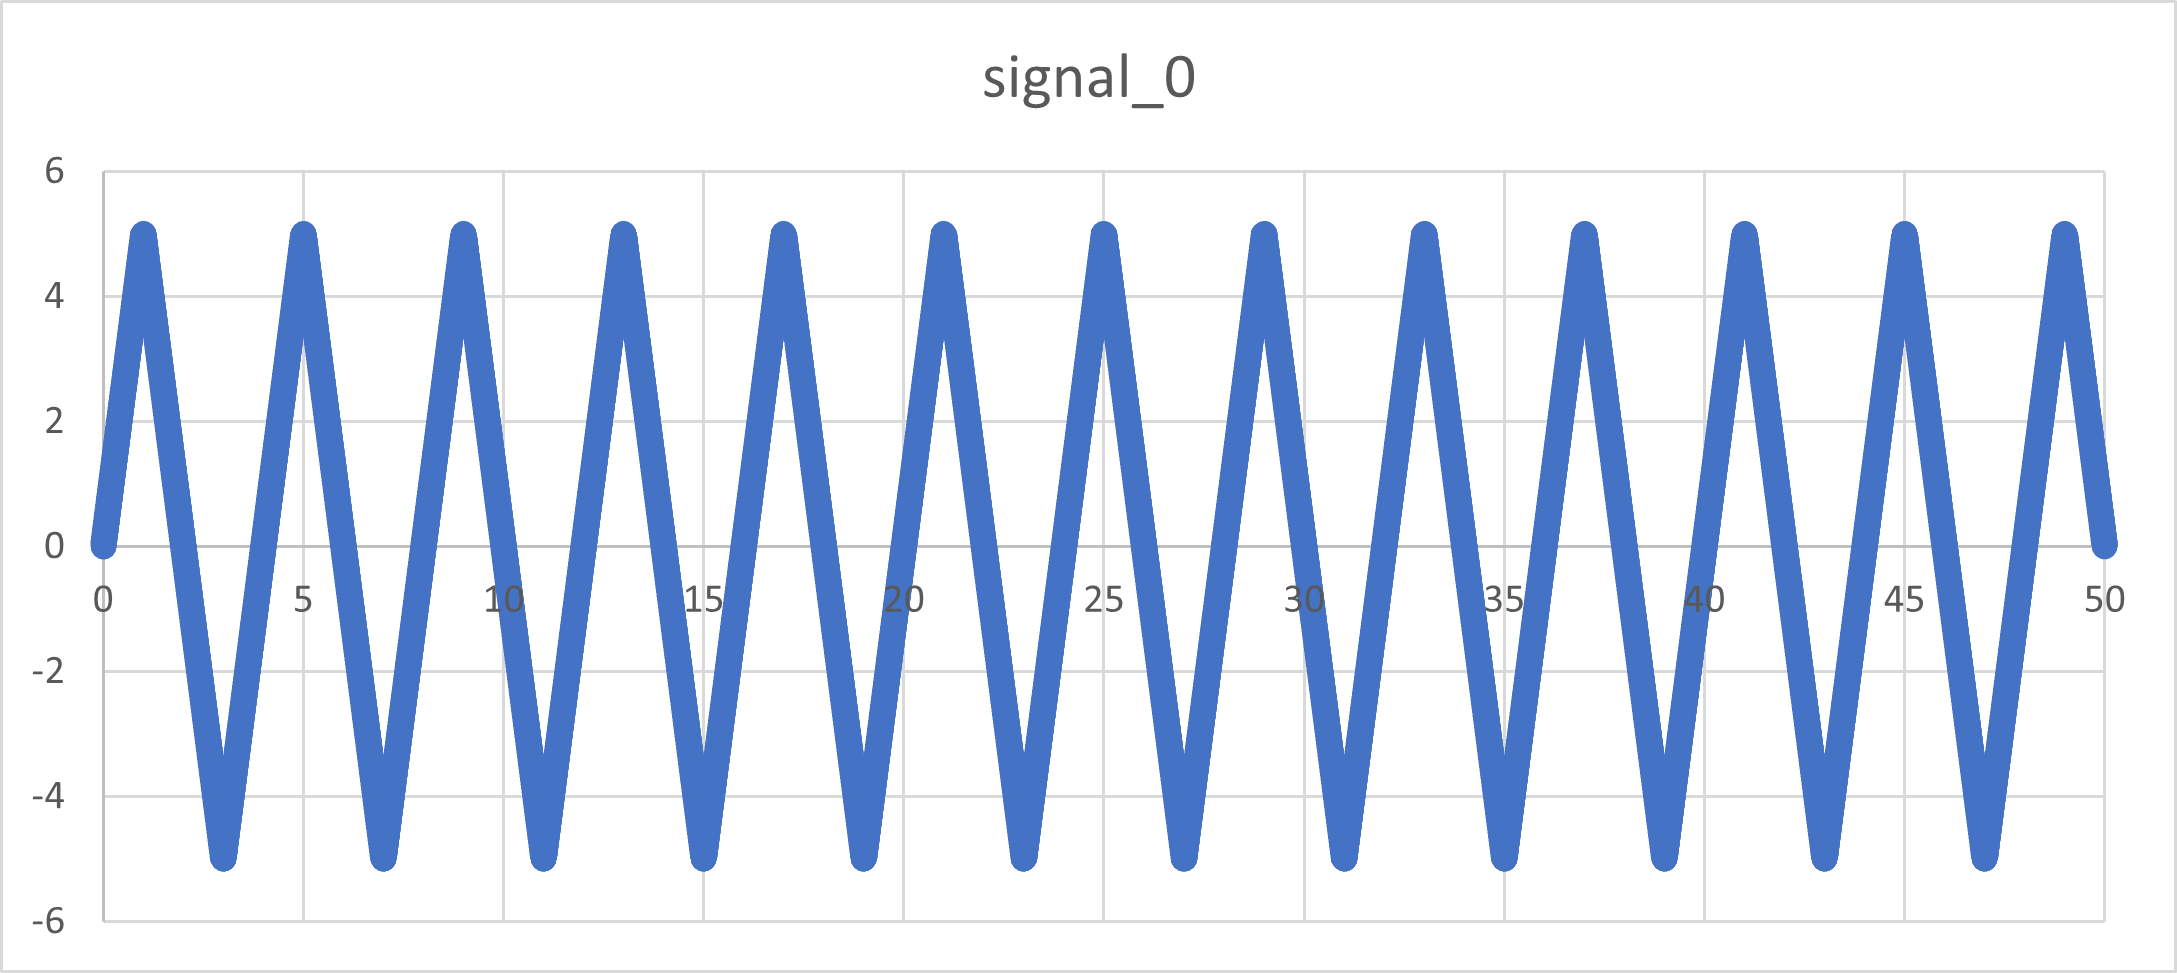
\includegraphics[width=0.7\linewidth]{images/triangular} 
\caption{Señal triangular}
\label{fig:trian}
\end{figure}

\begin{figure}[htb]
\centering
  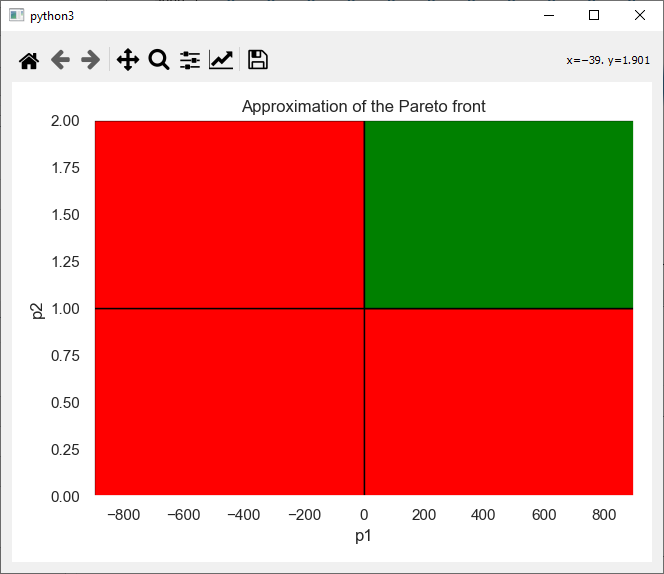
\includegraphics[width=0.7\linewidth]{images/stl_parametrico} 
\caption{Resultado paramétrico}
\label{fig:param}
\end{figure}
% Interfaz grafica
\chapter{Interfaz gráfica}
\label{cha:gui}

\section{Estructura}
Hasta ahora, las herramientas de verificación y minería mostradas en este proyecto utilizaban interfaces de usuario poco amigables para usuarios inexpertos: a través de línea de comandos para la herramienta STLEval, o mediante código fuente en Python para la biblioteca ParetoLib.

En este apartado proponemos un espacio donde el usuario tenga que simplemente adjuntar los ficheros de entrada con las señales y especificaciones, elegir la operación a realizar entre las opciones disponibles para finalmente visualizar y descargar los resultados en forma gráfica.

\begin{figure}[htb]
\centering
  \includegraphics[width=.95\linewidth]{images/uml_diagram}
\caption{Estructura del proyecto}
\label{fig:est}
\end{figure}

Tal y como vemos en la figura \ref{fig:est}, la nueva interfaz gráfica de usuario se comunica con la biblioteca de minería ParetoLib. ParetoLib nos permite evaluar propiedades con parámetros, utilizando en ese caso los métodos nativos de la biblioteca; o sin parámetros, redirigiendo la consulta a través de una adaptación de la interfaz anterior. A su vez, ParetoLib está conectado por el otro extremo a los binarios precompilados y la API de STLEval.

%La manera original de realizar las consultas a través de la terminal obligaba a hacerlas por separado a STLEval a la biblioteca de minería dependiendo si quisiésemos una consulta STL paramétrica o no.
Originariamente, el formato de las especificaciones en STL obligaba a interacturar con la herramienta STLEval o la biblioteca ParetoLib por separado según si las ecuaciones incluían parámetros o no (componente azul de la imagen).
La nueva interfaz gráfica de usuario unifica el proceso y facilita la usabilidad de cara al usuario.


Como aportaciones nuevas al proyecto (marcadas en rojo) está la propia interfaz gráfica de usuario, los operadores derivada e integral en STLEval y una modificación en la API paramétrica de STL, con la cual conseguimos ejecutar consultas no paramétricas desde ParetoLib.

\section{Bibliotecas utilizadas}

Debido a que la biblioteca ParetoLib está escrita en Python, y que con una pequeña modificación de la interfaz de interconexión permite acceder indirectamente a la API de STLEval, hemos decidido desarrollar la interfaz gráfica de usuario en ese mismo lenguaje. Para la elaboración de la parte gráfica de este proyecto hemos hecho uso de las bibliotecas:
\begin{itemize}
\item \href{https://www.qt.io/qt-for-python}{PyQt5}
\item Matplotlib
\item Pandas
\item Seaborn
\end{itemize}
 
\subsection{PyQt5}
La biblioteca PyQt5 está basada en la biblioteca gráfica Qt y sirve para realizar el diseño gráfico de la ventana principal de la aplicación desde Python. En nuestro caso optamos por un diseño simple de dos columnas: en la parte izquierda tenemos los botones y opciones para importar los ficheros de señales y la especificación de la operación, además de un espacio adicional para otras operaciones nuevas a implementar en un futuro. Al lado derecho tenemos la visualización de las señales tratadas y la especificación STL importada, la cual sólo se puede visualizar en modo lectura (es decir, los cambios en la especificación STL no se registrarán para la evaluación). Para extraer todo el potencial de PyQt5 hemos hecho uso de la herramienta \textit{Qt Designer}. Gracias a ella hemos podido construir el boceto de la interfaz, sobre la que después hemos anclado manualmente las funcionalidades a los botones correspondientes.

\begin{figure}[htb]
\centering
  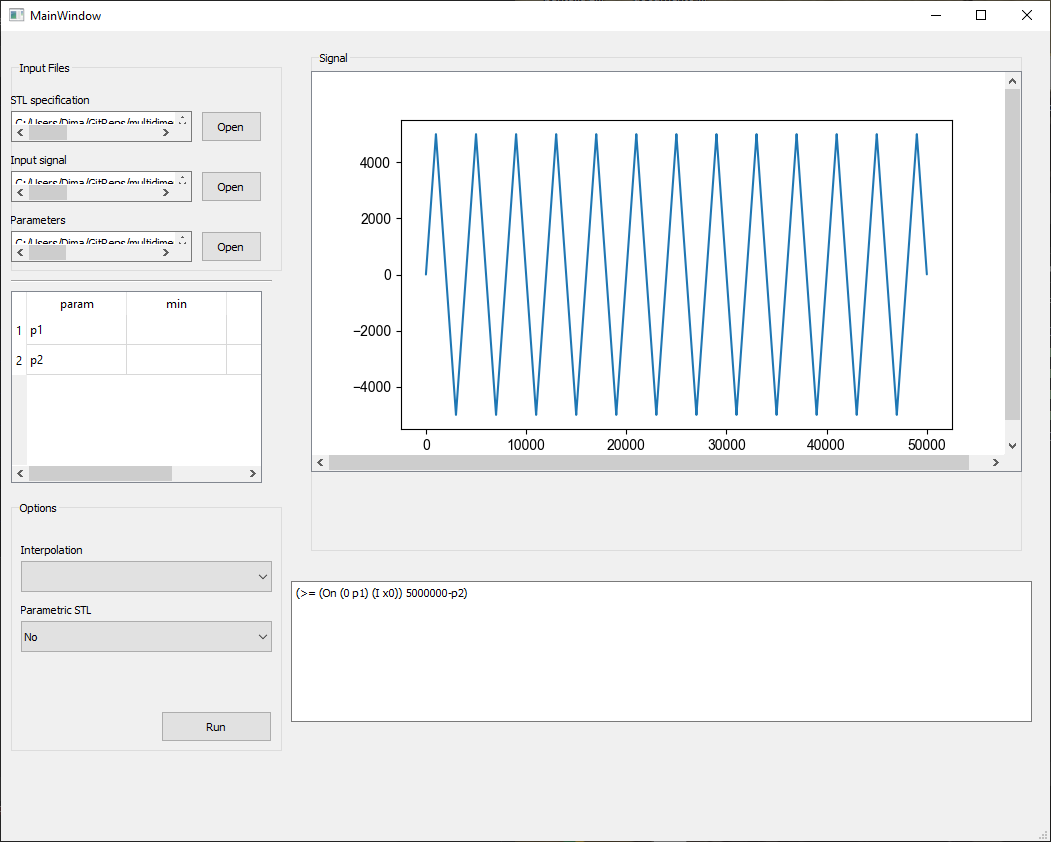
\includegraphics[width=1.0\linewidth]{images/gui} 
\caption{La ventana principal}
\label{fig:gui}
\end{figure}

%Instalación: 
%El desarrollo de la aplicación se hizo en un entorno linux haciendo uso del gestor de paquetes “pip”. 
 
%1 - Antes de todo, tenemos que confirmar la versión de Python que tenemos instalada con ´python3 --version´.
 
%2 - En el caso de que no lo tuviésemos, instalamos el gestor de paquetes “pip” con sudo ‘apt-get install python3-pip’ y actualizamos el mismo ´pip install -U pip´ 
 
%3 - Instalamos la librería PyQT con ´pip install pyqt5´. 
 
\subsection{MatplotLib}
La biblioteca MatplotLib da soporte a la mayoría de las bibliotecas gráficas avanzadas en Python (p.ej., Seaborn). Desde la versión inicial de ParetoLib, accesible únicamente a nivel de código fuente en Python, MatplotLib se utiliza para generar los gráficos resultantes de la minería de propiedades STL paramétricas (Figuras~\ref{fig:param_derivative}--\ref{fig:param_integral}). El uso del entorno PyQt5 para el diseño de la ventana principal de la nueva interfaz gráfica de usuario obliga a reajustar ligeramente la producción de estas imágenes de resultado para que se impriman dentro de una nueva ventana flotante en PyQt.
 
%Instalación: 
 
%1 - En este caso es sumamente simple realizando: ´sudo apt-get install python3-matplotlib´.
 
\subsection{Pandas}
La biblioteca Pandas es una biblioteca de Python especializada en el manejo y análisis de grandes bloques de datos. En nuestro caso, usamos esta biblioteca para la lectura lectura de las señales de entrada, las cuales están en ficheros csv y pueden albergar incluso miles de puntos.

Con esta biblioteca realizamos la transformación y almacenamiento de nuestras señales en una estructura de datos intermedia tipo \textit{DataFrame}, la cual utilizamos posteriormente como dato de entrada para los métodos de visualización gráfica de la señal a través de la biblioteca Seaborn.
 
%Instalación: 
 
%1 - Instalamos la librería con el comando: ´pip install pandas´

\subsection{Seaborn} 
Basada en MatplotLib, Seaborn es una biblioteca que permite generar fácilmente elegantes gráficos. Nosotros la utilizamos para dibujar las señales a partir de los datos importados en los archivos csv.

La función de esta biblioteca es meramente estética: creemos que este recurso es principalmente un añadido atractivo a la herramienta que puede ser útil en el caso que se quiera realizar presentaciones sobre sus resultados gráficos. Además, damos pie y esperamos poder realizar una mejora en todas las partes más visuales del aplicativo.
 
%Instalación: 
 
%1 - Instalamos la librería con el comando: ´pip install seaborn´

\section{Guía de uso}
En esta sección vamos a describir alguna de las partes interactuables o visibles de la interfaz gráfica de usuario:

\begin{itemize}
\item STL specification: Permite seleccionar un archivo \textbf{.stl}, el cual contiene una formula en STL (paramétrica o no). Cuando seleccionamos el archivo, la descripción de la formula aparece en una caja inferior en modo lectura (es decir, no modificable). Según si la consulta al motor de aprendizaje es paramétrica o no, habrá que modificar el casillero \textit{Parametric STL}.

\item Input signal: Permite seleccionar un archivo \textbf{.csv} que contiene la definición de la señal. Una vez seleccionado aparece un dibujo de esta en la caja grande de la ventana.

\item Parameters: Permite seleccionar un archivo \textbf{.param} que contiene los parámetros a estudiar y que aparecen en la formula del archivo .stl seleccionado. Es un fichero opcional: para una consulta no paramétrica no hace falta seleccionar ningún archivo. Al elegir un archivo, aparecerá más abajo una caja donde se deberá rellenar el intervalo de búsqueda (valores mínimo y máximo) de cada parámetro sobre los que la biblioteca de ParetoLib realizará el aprendizaje.

\item Parametric STL: Permite seleccionar si evaluaremos una consulta STL paramétrica o no: en el caso de quererla, seleccionamos que sí y viceversa.

\item Run: Permite ejecutar la consulta. Para poder hacerla necesitamos los tres ficheros de entrada anteriores descritos (dos ficheros en el caso no paramétrico). El clic de este botón recoge las rutas de los ficheros de entrada, el rango de valores numéricos de los parámetros (en el caso de haberlos) y prepara la invocación a la biblioteca de minería de forma similar al código mostrado en el código fuente \ref{list:paretolib_example}. En el caso de ser una consulta paramétrica, se nos devolverá un mapa con las regiones falsas o verdaderas según los parámetros (Figuras~\ref{fig:param_derivative}--\ref{fig:param_integral}). En el caso contrario, si la consulta no es paramétrica, simplemente devolverá el resultado de la evaluación: \textit{True} o \textit{False} (Figura~\ref{fig:noparam}).
%\textit{True} \ref{fig:noparam_true} o \textit{False} \ref{fig:noparam_false}.
\end{itemize}

%\begin{figure}[htb]
%\centering
%  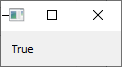
\includegraphics[width=0.3\linewidth]{images/stl_noparam_true} 
%\caption{Resultado no paramétrico True.}
%\label{fig:noparam_true}
%\end{figure}
%
%\begin{figure}[htb]
%\centering
%  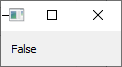
\includegraphics[width=0.3\linewidth]{images/stl_noparam_false} 
%\caption{Resultado no paramétrico False.}
%\label{fig:noparam_false}
%\end{figure}

\begin{figure}
\centering
  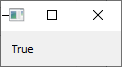
\includegraphics[width=0.3\linewidth]{images/stl_noparam_true} \hfill
  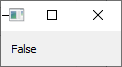
\includegraphics[width=0.3\linewidth]{images/stl_noparam_false} 
\caption{Resultado no paramétrico.}
\label{fig:noparam}
\end{figure}
% Conclusiones
\chapter{Conclusiones}
\label{cha:concl}
Para acabar este trabajo presentamos algunas conclusiones sobre los temas tratados, tanto teóricos como prácticos, y discutimos algunas ideas propicias para la mejora y continuidad del proyecto.
\section{Conclusiones (español)}

% Contribuciones
%En este proyecto, hemos actualizado los binarios y librerías dinámicas de STLEval que incorpora ParetoLib para dar soporte a las nuevas operaciones de derivación e integración. Además, hemos implementado una interfaz gráfica que abstrae la complejidad de invocar al código fuente ~\ref{list:paretolib_example} y resume la mayor parte de las opciones de configuración del algoritmo de minería.
Este TFG tiene como objetivo mejorar, diseñar, extender e implementar las herramientas STEval y ParetoLib para el tratamiento de señales aplicando la lógica temporal.

Durante el estudio realizado antes de trabajar en la extensión de las herramientas, hemos podido comprobar el arduo trabajo que llevan a cabo los investigadores de todas las materias para poder conseguir resultados y/o conclusiones que presentar, esta experiencia nos ha permitido valorar mucho más de lo que creíamos el esfuerzo y la labor de investigación de todos los profesionales, además de darnos  la satisfacción de poder tener este papel de investigadores en una versión más minúscula pero suficientemente retadora para nosotros. 

Como parte ya de la resolución del proyecto llegamos a extender las capacidades de la lógica temporal en la herramienta STLEval añadiendo las propiedades de la derivada, esto nos permitió comprender cómo  la recogida de datos unida a esta función matemática es capaz de mostrarnos tendencias y éstas son las que, actualmente, estamos viendo que van ganando más terreno tanto en los negocios como en nuestras vidas; y por otra parte la integral que se encarga de ... .Desde la aplicación creada se puede dar uso a éstas operaciones sin tener que pasar por la consola como en un principio ocurría.

Por otro lado, después de encargarnos de la implementación, aprendimos cómo conectar 2 herramientas que no estaban escritas en el mismo lenguaje de programación, esta tarea aunque al principio bastante complicada debido a que nunca antes la realizamos, la pudimos completar gracias a la ayuda de nuestro tutor quien siempre nos ofreció su ayuda, muchas veces incluso fuera del horario laboral. Además de esta integración actualizamos los binarios y librerías dinámicas de STLEval que incorpora ParetoLib para dar soporte a las nuevas operaciones de derivación e integración. 

Nuestra aplicación no dispone de una base de datos al trabajar con la propia y diferente información que va a tratar el usuario, es responsabilidad suya poseerla.

Para finalizar hemos implementado una interfaz gráfica que abstrae la complejidad de invocar al código fuente ~\ref{list:paretolib_example} y resume la mayor parte de las opciones de configuración del algoritmo de minería.


\section{Trabajo futuro}

Incluir más opciones en la GUI que nos permitan configurar parámetros adicionales de ParetoLib: p.ej., (des)activar el paralelismo, precisión del aprendizaje (EPS, DELTA, STEPS) ...

Actualmente STLEval sólo soporta interpolación constante. Como trabajo futuro, se plantea extender dicha herramienta para soportar nuevos tipos de interpolación (lineal, splines, etc.). Esto abre la posibilidad de desarrollar nativamente nuevos tipos de operadores lógico-temporales que permitan realizar predicciones sobre el futuro en base a unas señales ya conocidas y recogidas del artefacto que queramos monitorizar (aproximación mediante series de Taylor, análisis estadístico de las trazas u otros métodos de aprendizaje).

Implementar un procesador de lenguaje natural que facilite la escritura de expresiones en STL en un formato más agradable. P. ej.:
\begin{itemize}
 \item ``En el futuro, la propiedad X se cumple''
 \item ``F G (v > 120)'' en lugar de ``(F (G ( > v 120) )''
\end{itemize}

Reimplementar el núcleo de ParetoLib para aumentar las prestaciones computacionales: Python se puede compilar en lugar de interpretar, lo que aumentaría el rendimiento de la librería de minería. La mejora sería mínima (ParetoLib llama a STLeval para la mayoría de los cálculos, y STLeval está en C++), pero la mejora del rendiento al compilar Python nos ayudaría ahorrar unos pocos milisegundos.

\section{Conclusions (English)}
In view of the results of the previous chapter, $\ldots$



\chapter{Conclusions and future work}
\label{cha:concl_en}
To finish this project, we present some conclusions on the topics covered, both theoretical and practical, and we discuss some ideas that are conducive to the improvement and continuity of the project.

\section{Conclusions}
This project has aimed to improve the analysis capabilities of the tools for the verification of cyber-physical systems at runtime. To do this, we have used temporal logic as a formalism to specify the properties that the system must satisfy. In particular, we have used Signal Temporal Logic (STL, a type of temporal logic focused on the analysis of analog signals coming from physical sensors (i.e., speed or temperature).

Among the most relevant results in this project, we have managed to extend the capabilities of STL temporal logic to express properties that involve \textit{trends} (derivatives), or \textit{accumulations} (integrals). We have implemented these new logical operators in the current verification software tools, mainly in the STLEval tool. Along with STLEval, we have also taken care of the ParetoLib library, a mining library that learns (in)valid configurations of the monitored system, expressed as templates or parametric specifications in STL. ParetoLib internally interfaces with STLEval to perform calculations, so it has received an update to the STLEval binaries and DLLs that it packages together with the rest of the library to support the new derivation and integration operations.

Lastly, we have provided a friendly user interface that makes it easy to interact both with the learning library and indirectly with the STLEval tool. The graphical interface abstracts the complexity of invoking STLEval via the command line, or via Python source code in the case of ParetoLib (source code~\ref{list:paretolib_example}), as has been the case up until now. The graphical interface summarizes most of the configuration options of the verification tool and the mining algorithm.

Finally, we would like to emphasize the arduous effort made in the documentation and previous bibliographical research for the acquisition of the necessary knowledge for the elaboration of the results presented in these conclusions.

\section{Future work}
As future work, we propose the following extensions or improvements. On the one hand, we propose to include more options in the graphical user interface that allow us to configure additional parameters of the verification and mining tools and that have been omitted until now. For example, we will incorporate new fields to select the degree of precision of the learning, the level of parallelism in the calculations in ParetoLib or other possible choices from the source code in Python.

%(variables EPS, DELTA, STEPS)

On the other hand, currently STLEval only supports constant interpolation to fill the space between two sample points. As future work, it is proposed to enrich this tool to support new types of interpolation (i.e. linear, polynomial, splines, etc.). This opens the possibility of natively developing new types of logical-temporal operators that allow making predictions about the future based on already known signals collected from the artifact that we want to monitor (Taylor series approximation, statistical analysis of the traces or other learning methods). A prototype of a new logical-temporal operator would be the operator \textit{probability} or $\mathbf{Pr}_{\sim \lambda}\varphi$, where $\sim \in \{<, \leq, \geq, >\}$ and $\lambda \in [0, 1]$.

Next, implementing a natural language processor will make it easier to write expressions in STL in a more pleasing format for inexperienced users. As a first approximation, it will simply rewrite the equations in a more readable format (i.e. $F\, G\, (v > 120)$ instead of $(F \, (G \, ( > v \, 120))$) to later allow in future versions write properties of the style \textit{``In the future, property X is true''}.

Lastly, reimplementing the core of ParetoLib will increase the computational performance of the library. Python offers mechanisms to compile the source code instead of interpreting it, which would increase the performance of the mining library. The improvement would be minimal (ParetoLib calls STLeval for most calculations, and STLeval is in C++), but the performance boost when compiling Python would help us save a few milliseconds.

\newpage

\addcontentsline{toc}{chapter}{Bibliografía}
\nocite{*}

\printbibliography

\end{document}